% Preamble - - - -
\documentclass[12pt]{article}
% Variables - - - -
\def\course{QSS 20}
\def\assignment{Initial Data Analysis}
\def\byline{Transit and the World Cup, Greater Boston MSA}
\def\me{Roshan Karim}
\ifx\byline\empty
\def\subject{\course}
\else \def\subject{\course: \byline}
\fi
% - - - - Variables
% Commands - - - -
\newcommand{\opscale}[2]{\xrightarrow{#1r_#2 \text{→ } r_#2}}
\newcommand{\opreplace}[3]{\xrightarrow{r_#1 #2r_#3 \text{→ } r_#1}}
\newcommand{\opitc}[2]{\xrightarrow{r_#1 \text{↔} r_#2}}
% - - - - Commands
% Default Packages - - - -
\usepackage[letterpaper, total={6.5in, 9in}]{geometry}
\usepackage{fancyhdr}
\setlength{\headheight}{16pt}
\usepackage{titling}
\usepackage{citation-style-language}
\cslsetup{style = american-sociological-association}
\addbibresource{../Literature Review/references.json}
\addbibresource{../Literature Review/references.bib}
\usepackage{xurl}
\Urlmuskip=0mu plus 1mu
\setlength{\emergencystretch}{2em}
\usepackage[pdftitle={\assignment},
    pdfsubject={\subject},
    pdfauthor={\me},
    pdfproducer={LaTeX},
    pdfcreator={LuaLaTeX},
    colorlinks,
    citecolor=black,
urlcolor=blue]{hyperref}
\usepackage{graphicx}
\graphicspath{{./images/}}
\usepackage{parskip}
\usepackage[all]{nowidow}
% - - - - Default Packages
% Unique Packages - - - -
\usepackage{amsmath}
\usepackage{txfonts}
\usepackage{fontspec}
\setmainfont{Charis SIL}
\usepackage{bm}
\usepackage{tikz}
\usepackage{pgfplots}
\pgfplotsset{compat=newest}
% - - - - Unique Packages
% Header - - - -
\pagestyle{fancy}
\lhead{\course: \assignment}
\chead{\me}
\rhead{\today}
% - - - - Header
% - - - - Preamble
\begin{document}
% Title - - - -
\begingroup
\centering
\ifx\byline\empty
\LARGE\assignment\\
\else\LARGE\assignment\\\large\byline\\[1.5em]
\fi
\endgroup
% - - - - Title
% Content - - - -
\section{Project Description}
For my final project in QSS 20, I will be using a combination of custom-collected real-time transit data and publicly available U.S. Census data.

\section{Research Question}
Based on my review of the literature, I propose the following research question:
How do mega-events impact socioeconomic disparities in public transportation?
I want to examine transit dependability before, during, and after the World Cup, looking at the `differrences-in-differences,' to examin whether mega-events exacerbate or remediate socioeconomic disparities in transportation.
I believe this relationship to be complex, sitting at the intersection of infrastructure investment, political access, and existing neighborhood inequities.
I will examine the impact of the 2026 FIFA World Cup on communities in the Greater Boston metropolitan statistical area.

\section{Data}
My overall project dataset will be a combination of private and public data.
I outline each set below.
\subsection{Private: MBTA General Transit Feed Specification (GTFS), Realtime}
I created this dataset as part of my work for Keolis Commuter Services.
It is a rolling archive of GTFS-realtime feeds, which show the arrival and departure time of every train from every station.
Unfortunately, I only collected data for the Commuter Rail, and not mainline MBTA, as this was the goal of my work project.
However, this dataset remains among most comprehensive and `raw' railroad performance data available to me.
Relevant fields include trip identifiers, route identifiers, station arrival and departure times, and scheduled station arrival and departure times.
One thing that makes this dataset particularly valuable is the ability to `see beyond the schedule.'
Many railroads add extreme schedule padding and then report only summary metrics like on-time performance.
These mask the true differences in performance day-to-day.
\subsection{Public: American Community Survey (ACS)}
\citet{allenSizingTransportPoverty2019} propose a simple yet robust model for overall neighborhood socioeconomic status (SES), defined by the following equation:
$$ I_\mu = \frac{1}{4}\hat{I}_{\ln \mathrm{MHI}} - \frac{1}{4}\hat{I}_{\mathrm{UR}} - \frac{1}{4}\hat{I}_{\mathrm{LIM}} - \frac{1}{4}\hat{I}_{\mathrm{LICO}}$$
Where $\hat{I}$ is the standardized score of each of the four measures: log of median after-tax income, unemployment rate, low income measure, and low income cut-off.
The last two, being specific Statistics Canada measures of poverty rates in a community, are not directly available but easily calculated from ACS data

\section{Initial Visualizations}
\subsection{Accrued Delay by Stop}
\begin{center}
    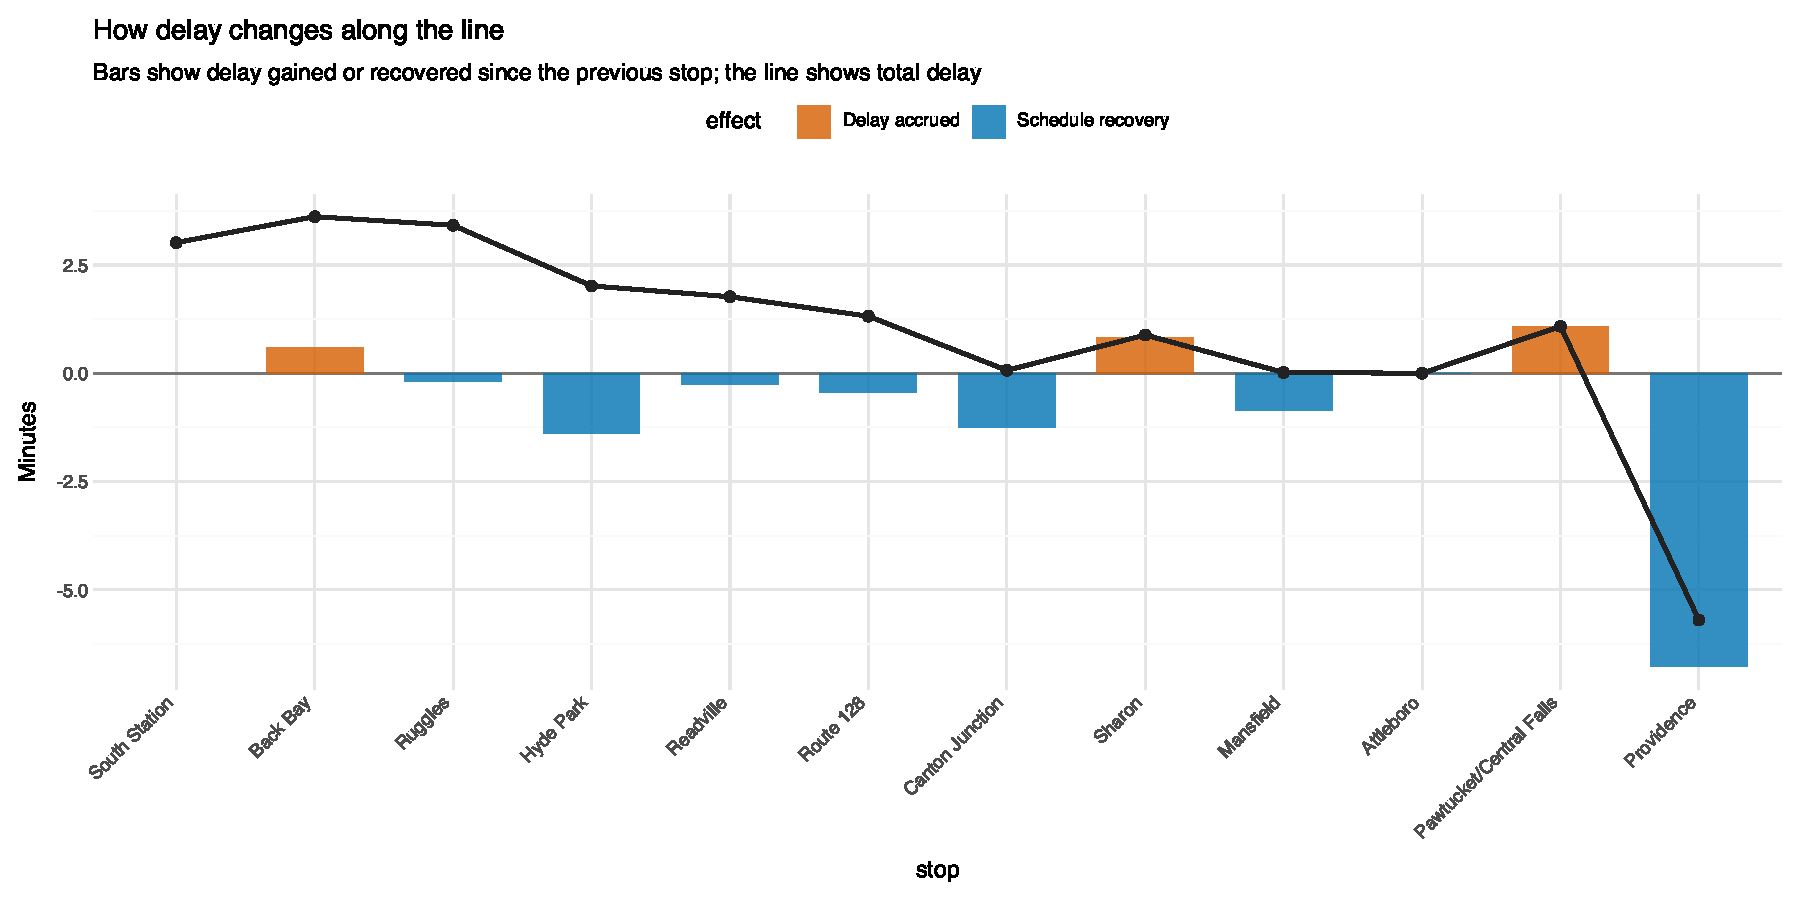
\includegraphics[width=6.5in]{../charts/delay_change_by_stop.pdf}
\end{center}
To demonstrate the importance of stop-by-stop data, I created a visualization to elucidate the effect of schedule padding.
This particular train demonstrates significant pad at the end stop, and likely some at Hyde Park as well.
Thus, it is not fair to judge transit dependability based simple on on-time performance.
It is necessary to examine arrival windows at each stop, especially since they serve different communities with different neighborhood SES.
\subsection{Neighborhood Socioeconomic Status}
\begin{center}
    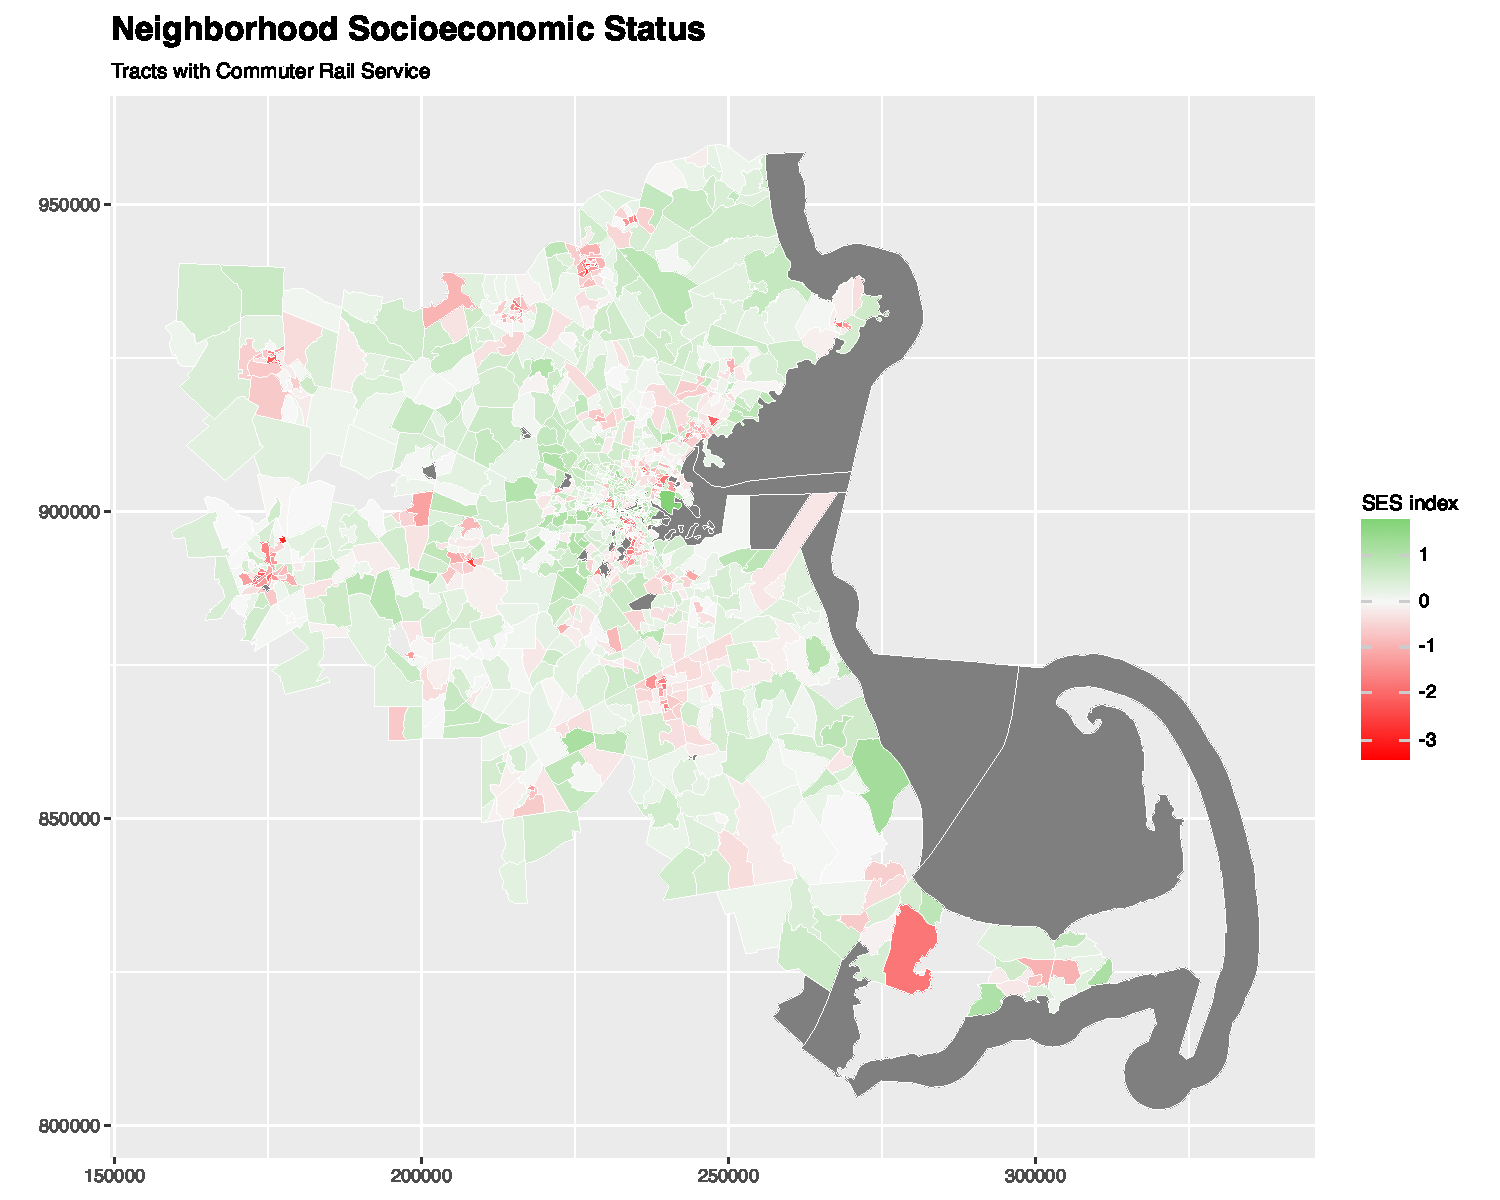
\includegraphics[width=5in]{../charts/ses_map.pdf}
\end{center}
This visual shows my chosen SES index metric over the neighborhoods in Greater Boston served by the Commuter Rail.
It was a necessary sanity check on SES calculations and is useful in its own right.

\section{Lessons from Prior Project}
The linked report demonstrates the importance of distinguishing statistical significance from substantive significance. 
The report found statistically significant coefficients for local COVID-19 cases and deaths, but the effects were essentially zero. 
This is a salient example of why researchers should interpret effect sizes rather than relying solely on statistics.

One weakness is that the authors used a simple pre-/post pandemic indicator to estimate the pandemic's effect.
This approach does not account for preexisting trends, seasonality, or other events.
It cannot support a causal interpretation.
Using time-series data, one could estimate the preexisting trend to improve causal understanding. 

\section{Challenges}
The first and primary challenge of my project is to wrangle the data.
The data downloaded from the MBTA is not particularly clean, with timestamp inaccuracies and missingness common.
Fixing this will require a lot of work, but it is a necessary first step.

The second challenge is to estimate anything approaching casual effects.
I don't believe that the data here is sufficient to do more than measure association between SES and transit dependability.
However, because of the natural experiment in the World Cup, it may be possible to estimate casual effects of mega-events, which is a priority.
% - - - - Content
\end{document}